\documentclass[a4paper,11pt]{article}
\usepackage{graphicx}
\usepackage[T1]{fontenc}
\usepackage[latin1]{inputenc}
\usepackage{graphicx}
\usepackage{titlesec}
\usepackage{xcolor}
\usepackage{amsfonts}
\usepackage{algorithm}
\usepackage{wrapfig}
\usepackage{algpseudocode}
\usepackage{wrapfig}
\usepackage{svg}
\usepackage{amssymb}
\usepackage{floatflt,epsfig}
\usepackage{subfigure}
\usepackage{multirow}
\usepackage{glossaries}
\usepackage{booktabs}
\newtheorem{theorem}{Theorem}
\newtheorem{lemma}{Definition}
\newtheorem{proposition}{Proposition}
\newtheorem{proof}{Proof}
\usepackage{tikz}
\tikzstyle{mybox} = [draw=black, thin, rectangle, rounded corners, inner ysep=5pt, inner xsep=5pt, fill=orange!20]

\usepackage[a4paper, top=2cm , bottom=2cm , right=1.5cm , left=1.5cm ]{geometry}

\begin{document}
    
    \title{
        \linespread{0.3}
        \vspace{-2.5cm}
        \textbf{
        {\large{MODELING AND CONTROL OF CPSs}  - \Large {Project activity report (Part I)}}\\
        %{\Large{Project Activity Report}}
        }
        \vspace{-0.5em}
    }
    \author{
        \textit{
            \normalsize 
        Lorenzo AGHILAR} \text{(334086)},
        \textit{Carlo MIGLIACCIO} (332937), 
        \textit{Federico PRETINI} (329152)}
    
    \date{}

    \clearpage\maketitle
    \thispagestyle{empty}
    \vspace{-2em}
    
    \vspace{-0.5cm}
\section*{Task \#1: IST algorithm for solving LASSO}

\subsection*{Brief theoretical introduction}
When we have to solve an optimization problem, finding a \textit{simple approximate solution} is surely better than an exact but  
more complex one. 
In our case \textbf{simplicity} corresponds to \textbf{sparsity}. A solution is said to be \textbf{sparse} if it has \textbf{few non-zero elements}. A \textit{sparse optimization problem} can be formultated in the form $ \min_{x\in X} \  f(x) \ \text{s.t.} \ \Vert x \Vert_0 \le h$, where $x$ is the optimization variable and $f(x)$ the objective function. The main disadvantage of this formulation is the $\ell_0$-norm which, being \textit{non-convex and discontinuous}, makes the problem itself \textbf{hard} to be solved. Here the trick is the use of the $\ell_1$-norm as an approximation, which has better properties, first of all the \textbf{convexity}.\\
%Sparse Optimization is ubiquitous since the found solutions are easier to store and implement. Just to give an example, in machine learning one can find useful a \textbf{sparse model} with few parameters in order to avoid problems related to the overfitting (the model is too much linked to the training data).\\
In many real-world applications we need to find a \textbf{sparse solution} to a large underdetermined systems of linear equations. The presence of \textbf{measurement noise} in collecting data justify us in using a least-squares approach while the requirement on sparsity is fulfilled by introducing an $\ell_1$-based penalty. This raises the problem of \textbf{LASSO} (\textit{Least Absolute Shrinkage and Selection Operator}) defined as
\vspace{-0.2cm}
\begin{equation} \label{eq:LASSO} 
    x^* = \text{arg} \min_{x \in \mathbb{R}^n} \frac{1}{2}\Vert y-Ax \Vert_2^2 + \lambda \Vert x \Vert_1, \ \lambda >0
    \vspace{-0.2cm}
\end{equation}
where $\lambda$ is an hyperparameter to tune. There are many algorithms to solve the LASSO problem. However, the objective of this task is to analyze the \textbf{Iterative Shrinkage/Thresholding Algorithm} also called \textbf{ISTA}.

\vspace{-0.2cm}
\subsection*{Iterative Shrinkage/Thresholding Algorithm}
The algorithm on which we focus our attention is derived from the \underline{alternating minimization} of a \textit{surrogate funtional} $\mathcal{R}(x,b)$ which is obtained adding some terms to the one in (\ref{eq:LASSO}). 
\begin{algorithm}
    \caption{Iterative Shrinkage and Thresholding Algorithm (ISTA)} \label{alg:ISTA}

    \vspace{0.3cm}
    \begin{enumerate}   
        \itemsep-0.3em
        \item  \textsf{\textbf{Initialization}} $x_0 \in \mathbb{R}^n$, e.g. $x_0=0$
        \item \textsf{For each $k=0, ..., T_{max}$}
        \vspace{-0.5cm}
        \begin{equation*}
            x(k+1)=\mathbb{S}_{\lambda\tau}[x(k)+\tau A^T(y-Ax(k))], \quad 
            \mathbb{S}_{\lambda\tau}=
            \begin{cases}
                x_i-{\lambda\tau} & \text{if $x_i$>${\lambda\tau}$} \\
                x_i+{\lambda\tau} & \text{if $x_i$ < -${\lambda\tau}$}\\
                0 & \text{if $ \lvert x_i \rvert \le \alpha$}\\ 
            \end{cases}
        \end{equation*}
        \vspace{-0.7cm}
        \item \textbf{\textsf{Stop condition}}: $\Vert x(T+1) - x(T) \Vert < \delta,\ \delta=10^{-12}$
    \end{enumerate}
\end{algorithm}


\noindent
 $\mathbb{S}_{\lambda\tau}$ is the \textbf{Shrinkage/Thresholding operator}.
 The parameter $\lambda$ has a crucial role, in particular for $\lambda=0$ we just get the LS estimate of the full model, while for \textit{very large} $\lambda$ the LASSO estimates are exactly zero.
The \textbf{Algorithm (\ref{alg:ISTA})} has the following properties: (i) it is a \textbf{descent algorithm}, (ii) it converges to the minimum of LASSO; furthermore, its iterative nature makes it suitable for both \textbf{dynamic} and \textbf{distributed} settings.
\vspace{-0.2cm}
\subsection*{Analysis and Results}
In order to perform the analysis, data have been randomly generated: the entries of $C$ are distributed according $\mathcal{N}(0,1)$;  the entries of the (sparse) vector $x$ are assumed to be uniformly distributed; finally the solution is imposed to be 2-sparse. The \textbf{measurement phase} is distributed in the sense that the measurements have to be interpreted as taken by $q$ sensors, each one of them taking one measurement.
\subsubsection*{First aspect: Support recovery rate}
The \textbf{support} of a solution is the set of indexes at which the non-zero elements are placed. The analysis is performed on what is the \textbf{effect of increasing the number of sensors $q$} in the capability of the algorithm in recover correctly the support of the solution. To this aim, for each value of $q$ from 5 to 20, 20 experiments have been executed.
\begin{figure}[h]   
    \vspace{-1cm}
    \centering 
    \subfigure[Support recovery rate]
    {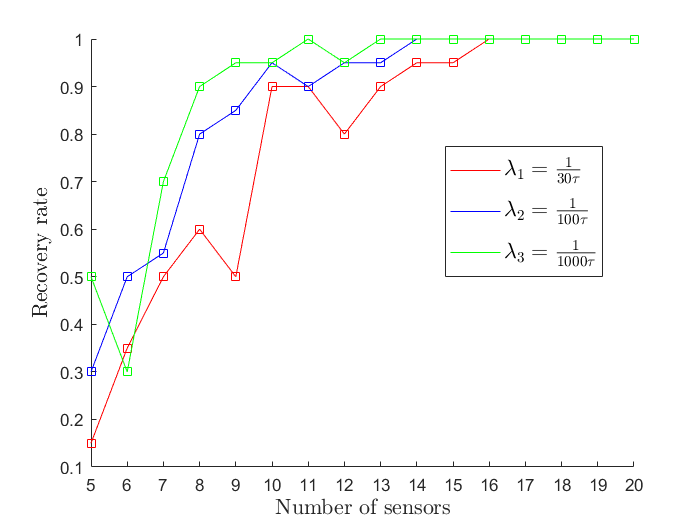
\includegraphics[scale=0.3]{img/SuppRecRate.png}}
    \subfigure[Convergency time (I)]
    {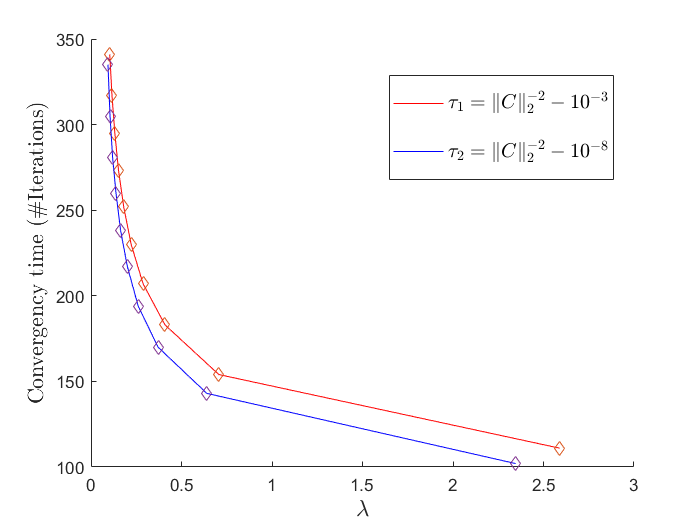
\includegraphics[scale=0.3]{img/Conv_lambda.png}}
    \subfigure[Convergency time (II)]
    {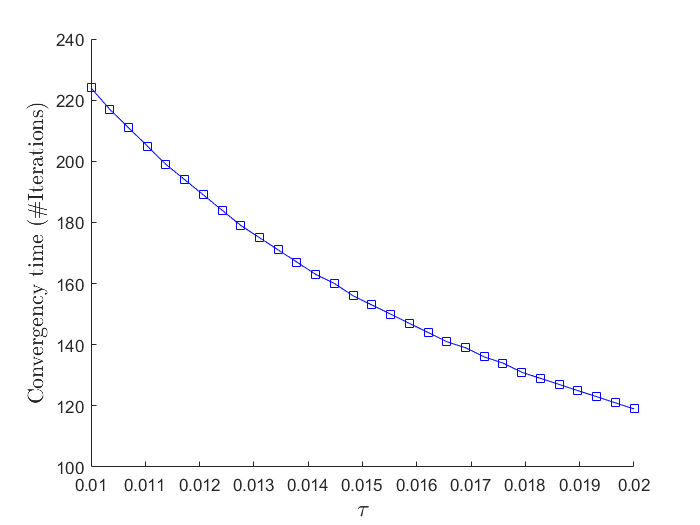
\includegraphics[scale=0.3]{img/conv_tau.png}}
    \caption{Results for the analysis of ISTA}
    \label{fig:Results}
\end{figure}

It can be observed Figure (\ref{fig:Results}a) that increasing the number of sensors the support recovery rate improves reaching also 100\% for $13\le q \le6$. Moreover the experiments have been repeated for three different and decreasing value of $\lambda$. 

\subsubsection*{Second aspect: Convergence time}

The objective here is to discuss how the hyperparameters $\tau$ and $\lambda$ can affect the performances of ISTA in term of \textbf{convergency time}, which - for our purposes - is the \textbf{number of iterations} needed to meet the stop condition. Two different types of experiments have been carried out: the first aimed to explain what happen when we change the coefficient $\lambda$ of the regularization and keeping $\tau$ constant, the second in order to change $\tau$, keeping $\tau\lambda$ constant, and see the related effects.\\
\vspace{-0.4cm}
\begin{table}[h] \label{table:1}
    \centering
    \begin{tabular}{| p{2cm} || p{1cm} |p{1cm} |p{1cm} |p{1cm} |p{1cm} |p{1cm} |p{1cm} |p{1cm} |p{1cm} |p{1cm} | }
        \hline
        $\boldsymbol{\lambda}$&0.0800&0.0896&0.1017&0.1177&0.1396&0.1715&0.2223&0.3160&0.5457&2.0011\\
        \hline
        {\color{blue}Iterations}  &621&590&560&529&456&404&367&328&287&236\\
        \hline
        {\color{red}Iterations}  &647&617&586&518&477&423&386&347&306&253\\
        \hline    
    \end{tabular}
    \caption{Convergency time in function of $\lambda$}
    \vspace{-0.3cm}
\end{table}

\noindent
How can be noted from the Figure (\ref{fig:Results}b), when we use an higher $\lambda$ the convergency time is smaller. This is due to the fact that a larger $\lambda$ drives faster the elements of the solution of the problem (\ref{eq:LASSO}) close to zero, in this way the stop criterion is met sooner. However, the graph in (1a) shows that the performance in term of support recovery rate is worst on average. More detailed information can be found in Table (1).\\
On the other side, we have a similar situation when $\tau$ (step-size) is the parameter being changed: an higher $\tau$ leads to a faster convergence, this is related to the fact that in this case the distance between solution $x(T+1)$ and $x(T)$ for a generic instant $T$ is larger. Figure (\ref{fig:Results}b) shows that keeping $\lambda$ constant, if we choose  {{\color{red}$\tau_1$} $<$ {\color{blue}$\tau_2$}} the convergency time is on average higher. Finally the Figure (1c) shows the evolution of the number of iterations keeping the product $\tau\lambda$ constant.

\subsection*{Conclusion}
We can conclude that the parameter $\lambda$ is crucial for the solution of the LASSO problem since such a parameter drives it to be more or less sparsified. In particular, if lambda is too small the found solution tends to the one of the "full model" (Least-Squares) which is not sparse at all and will not satisfy the requirement on simplicity we have made at the beginning, however the convergence time is smaller; on the other side if lambda is too small the solution we get is closer and closer to the zero element of  $\mathbb{R}^n$, deriving an estimate, as solution of the optimization problem, which is too much "sparsified"; the convergence time is higher than the previous case. At this point one can understand that a \textbf{trade-off between convergence time and performance} (support recovery rate) has to be managed.



       % Carlo Migliaccio

    %\section*{Task \#2: Secure State Estimation of CPSs}

\subsection*{Brief theoretical introduction}

%----------------------------------------------
\subsection*{Algorithm}

%----------------------------------------------
\subsection*{Results}


\subsubsection*{Aspect 1}

\subsubsection*{Aspect 2}
%----------------------------------------------       % Lorenzo Aghilar

    %\section*{Task \#3: Localization under sparse sensor attacks}

\subsection*{Brief theoretical introduction}

%----------------------------------------------
\subsection*{Algorithm}

%----------------------------------------------
\subsection*{Results}


\subsubsection*{Aspect 1}

\subsubsection*{Aspect 2}
%----------------------------------------------       % Lorenzo Aghilar
    
    %materiale vecchio: ho spostato qui per sicurezza nel caso ci fosse qualcosa di utile da recuperare
%                   Carlo

\section*{Task \#4: Dynamic SSE}
    \subsection*{Introduction}
    In the previous task we performed SSE on a static system, now we leave out the static hypothesis and move into the dynamic one.
    In the dynamic setting the martix A is no longer the identity matrix and in order to solve this problem we couldn't use least square or Gradient Descent (GD) algorithms due to their performances. Instead we run a single GD step at each $k$ instant, this algorithm has been called the Online Gradient Descent or \textbf{OGD} and is used to develop a sparse observer
    
    \subsection*{Algorithms}
    The algorithm of the sparse observer is the following:
    \\Given $y(k) = Gz(k)$ and $\hat{z}(k)$
    \begin{equation} \label{eq:OGD}
        \begin{aligned}
            &\hat{z}^+(k) = \hat{z}(k) - \tau G^T[G\hat{z}(k) - y(k)]\\
            &\hat{x}(k+1) = A\hat{x}^+(k)\\
            &\hat{a}(k+1) = \mathbb{S}_{\tau \lambda}[\hat{a}^+(k)]\\
            &\hat{y}(k) = G \hat{z}(k)\\
        \end{aligned}    
    \end{equation}   
    
    \subsection*{Results}
    Below are the results presented in the following structure:
    \begin{itemize}
        \item Image: the image is further divided into two parts. On the left side $(a)$, a specific case of the results obtained by the execution of the algorithm after T time instant is shown, while on the right side $(b)$, the final situation of the room is presented, providing a snapshot of the SSE result after T time instants.
        \item Table: a summary table that gives information on the results obtained by running the algorithm 100 times under the same conditions in terms of: targets,sensors under attack,execution time ($T_{max}$) and type of attack carried out. This table is useful to understand how the algorithm generally behaves.
    \end{itemize}
\noindent
    The convergence of the attack $a$ and state $x$ are understood as a match between the support of the actual vector and the estimated vector. For the observer insted the convergence time is understood as intersection between the convergence of the two previous vector.
    \subsubsection*{Main task: unaware attack}
    Using $\Lambda = [10,...10,20..20]$, a time simulation of 50 and matrices $A,D,Y$ provided by the file $tracking\_moving\_targets.mat$ we obtain that in general the sparse observer converge in 34 time instants and in particular the positions of the targets are correctly estimated only after 23 time istants.
    \begin{figure}[h]
    \centering
    \subfloat[Convergence]{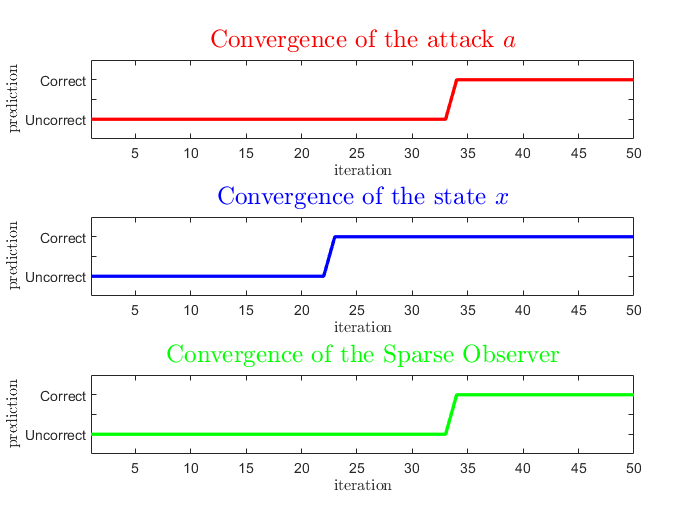
\includegraphics[width=.40\linewidth]{img/unaware_2.png}}
    \subfloat[Room]{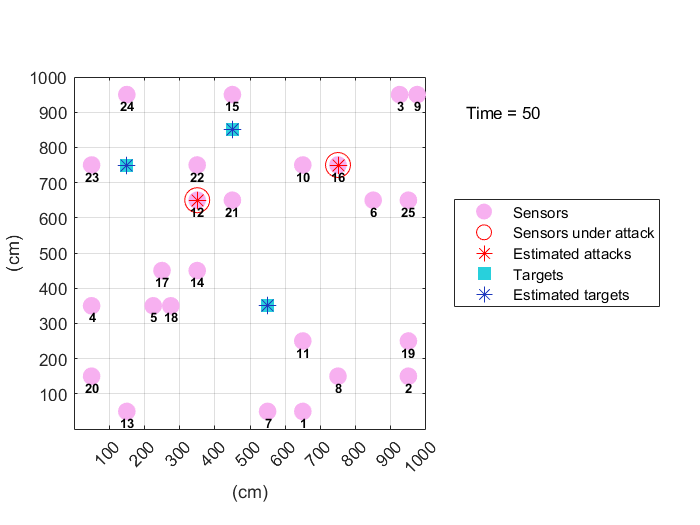
\includegraphics[width=.40\linewidth]{img/unaware_1.png}}
    \caption{Unawere: Three targets and two sensors under attack}
    \end{figure}
    
    \noindent
    In this case the table was not reported because it would not add any additional information since the matrices used are always the same. In fact even running the algorithm 100 times we always get observer convergence with convergence times of the attack estimate of 34 time instants and 23 for the state

    
    \newpage
    \subsubsection*{1\# optional task: aware time-varying attack}
    For this first optional task, the A and D matrices are always the same while the Y matrix was computed starting from randomly generated initial conditions. At each time instant $k$ an attack equal to half the previous value of the output is injected on the actual output ($a(k)= \frac{1}{2}y(k-1) \forall k=1..50$). 
      \begin{figure}[h]
    \centering
    \subfloat[Convergence]{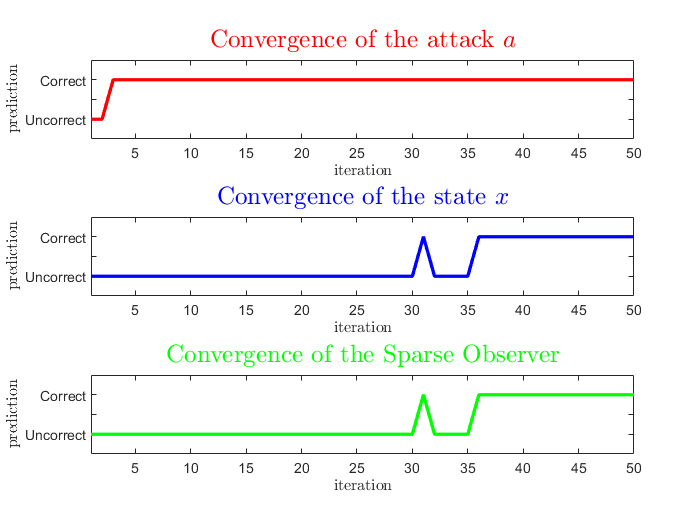
\includegraphics[width=.40\linewidth]{img/aware_2a_3x_2.png}}
    \subfloat[Room]{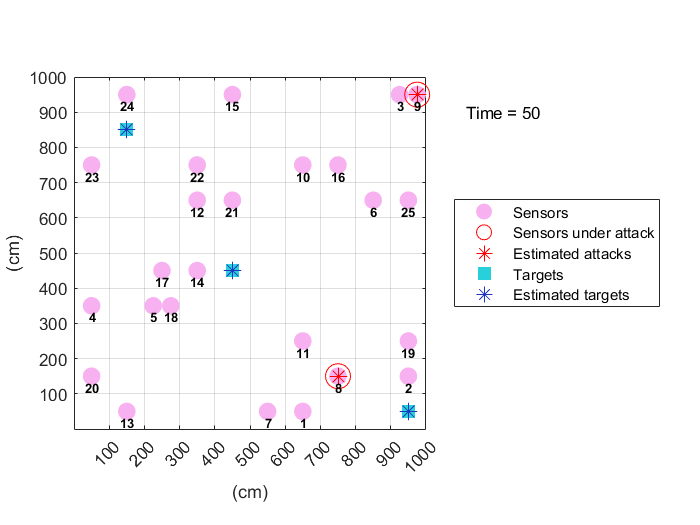
\includegraphics[width=.40\linewidth]{img/aware_2a_3x_1.png}}
    \caption{Aware: Three targets and two sensors under attack}
    \end{figure}
    
\noindent
As can be seen, in general, the sensors under attack are always correctly identified. However, regarding the position of the targets, only in 87\% of the cases, after 50 instant of time, a correct estimate is achieved.
    
\begin{table}[h!]
\centering
\begin{tabular}{|c|c|c|}
\hline
\multirow{2}{*}{\textbf{For 100 iterations}} & \multicolumn{1}{|c|}{\textbf{attack $a$}} & \multicolumn{1}{|c|}{\textbf{state $x$}} \\
\cline{2-3}
 & \textbf{1-50} & \textbf{1-50}\\
\hline
\textbf{\% convergence} &98\% &89\%  \\
\hline
\textbf{Mean time of convergene} &4.29 &30.46 \\
\hline
\textbf{Minimum time of convergence} &2 &10  \\
\hline
\textbf{Maximum time of convergence} &13 &50 \\
\hline
\textbf{Temporay loss of tracking} &2\% &58\%  \\
\hline
\end{tabular}
\caption{Summary table showing some statistics on $a$ and $x$}
\label{table:1}
\end{table}
            
    \subsubsection*{2\# changing sensors under attack}
For the second task, an additional complication was introduced by changing the sensors under attack every 25 instant of time. In the graph shown in the figure, it can be seen that, in general, this change of sensors under attack causes problems in tracking the targets, temporarily shifting the state prediction from correct to incorrect. In most cases, by the end of the 50 instants of time, the state is still correctly recovered.
    \begin{figure}[h]
    \centering
    \subfloat[Convergence]{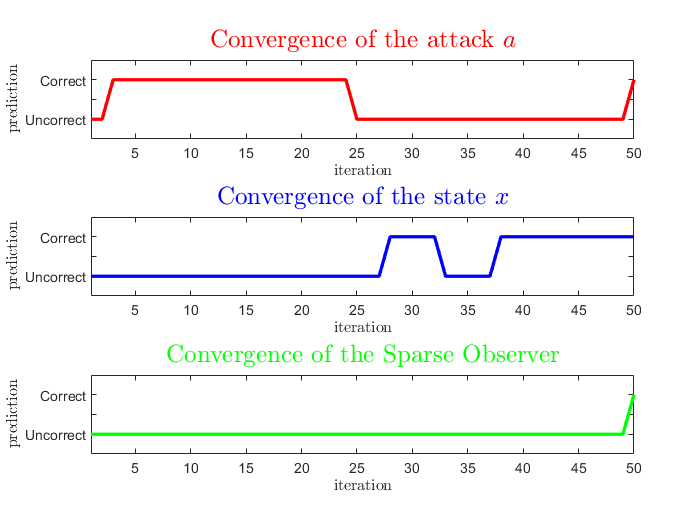
\includegraphics[width=.40\linewidth]{img/aware_2a_3x_cs_2.png}}
    \subfloat[Room]{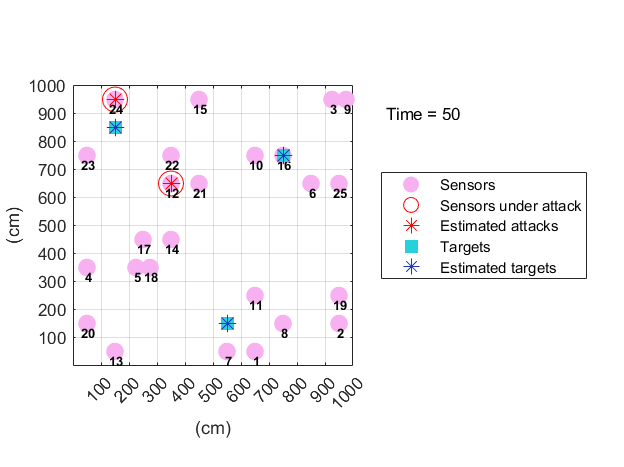
\includegraphics[width=.40\linewidth]{img/aware_2a_3x_cs_1.png}}
    \caption{Aware: Three targets and two sensors under attack}
    \end{figure}
\begin{table}[h!]
\centering
\begin{tabular}{|c|c|c|c|}
\hline
\multirow{2}{*}{\textbf{For 100 iterations}} & \multicolumn{2}{|c|}{\textbf{attack $a$}} & \multicolumn{1}{|c|}{\textbf{state $x$}} \\
\cline{2-4}
 & \textbf{1-25} & \textbf{26-50} & \textbf{1-50} \\
\hline
\textbf{\% convergence} &99\% &76\% &80\% \\
\hline
\textbf{Mean time of convergene} &4.71 &45.73 &36.16 \\
\hline
\textbf{Minimum time of convergence} &2 &36 &12 \\
\hline
\textbf{Maximum time of convergence} &16 &50 &50 \\
\hline
\textbf{Temporay loss of tracking} &6\% &1\% &62\% \\
\hline
\end{tabular}
\caption{Summary table showing some statistics on $a$ and $x$}
\label{table:2}
\end{table}
    
    \subsubsection*{3\# optional task: Maximum number of sensors under attack}
    To determine the maximum number of sensors under attack, a convergence threshold of at least 50 percent was cosidered for both state x and attack a for both 100 simulation in a time period of 100. A maximum number of sensors under attack was found to be 7 with 5 targets to be tracked.
    \begin{figure}
    \centering
    \subfloat[Convergence]{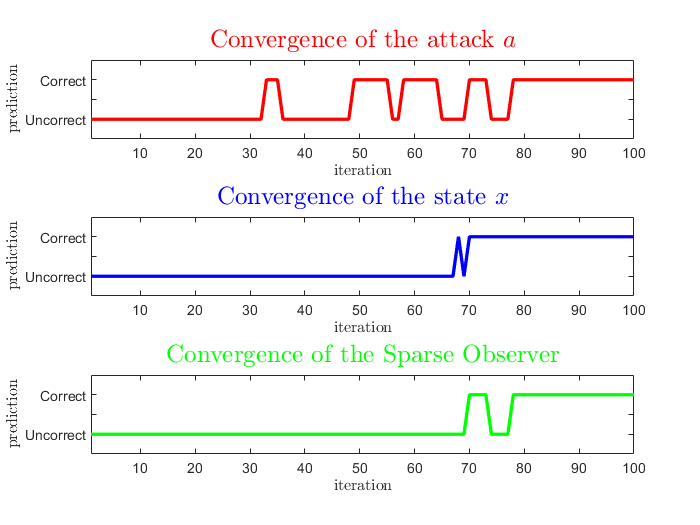
\includegraphics[width=.40\linewidth]{img/aware_7a_5x_2.png}}
    \subfloat[Room]{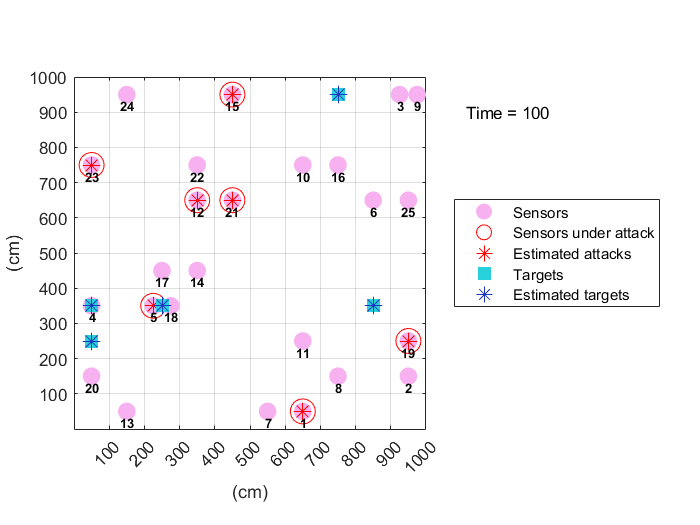
\includegraphics[width=.40\linewidth]{img/aware_7a_5x_1.png}}
    \caption{Aware: Five targets and seven sensors under attack}
    \end{figure}
\begin{table}[h!]
\centering
\begin{tabular}{|c|c|c|}
\hline
\multirow{2}{*}{\textbf{For 100 iterations}} & \multicolumn{1}{|c|}{\textbf{attack $a$}} & \multicolumn{1}{|c|}{\textbf{state $x$}} \\
\cline{2-3}
 & \textbf{1-100} & \textbf{1-100}\\
\hline
\textbf{\% convergence} &51\% &59\%  \\
\hline
\textbf{Mean time of convergene} &41.76 &71.64 \\
\hline
\textbf{Minimum time of convergence} 6 &27  \\
\hline
\textbf{Maximum time of convergence} &100 &99 \\
\hline
\textbf{Temporay loss of tracking} &32\% &37\%  \\
\hline
\end{tabular}
\caption{Summary table showing some statistics on $a$ and $x$}
\label{table:3}
\end{table}


    
    \subsection*{Additional comments}
    For data cleaning, we used prior information about the number of targets, whereas for the number of sensors under attack, we used a threshold. This is because, in reality, assuming knowledge of the number of sensors under attack is not plausible. Specifically, we assumed that if the estimated attack on a sensor was below 50\% of the highest recorded value at that moment for all sensors, then that value would be set to zero. Of course, this approach yields worse performance compared to filtering the data with knowledge of the number of sensors under attack, but it is also the most realistic.
       % Federico Pretini

    %\pagebreak
\section*{Task \#5: Distributed Secure State Estimation of CPSs}

\subsection*{Brief theoretical introduction}
The framework in which CPSs are located is intrinsically \textbf{distributed}, for this reason we move in the direction of \textit{fusion center removal} and the use of a distributed approach also for computation; this is done by using \textbf{distributed algorithms} which requires the devices of the CPS modeled as a multi-agent systems to 
%The motivation for \textbf{decentralization} is quite practical: a large number of cheap interconnected devices is better than few expensive devices. In this part we refer to a general CPS as a \textbf{multi-agent system}, in a nutshell a collection of devices which cooperate in order to reach a \textbf{common goal}, which for our purposes is the \underline{secure state estimation (SSE) of a dynamical system}.
cooperate, in the sense that they have to exchange some information through a communication network which is modeled by a digraph. 
Important results on \textbf{Consensus algorithm} guide us in the choice of the type of information to be shared: the local estimate $x^{(i)}(k)$ of the state. Under certain condition by iterating the computation of a \textbf{local quantity}, a global estimation $x^*$, equal for all the agents (the consensus), can be reached.
The ideas on which Consensus algorithm is based can be exploited for the minimization of composite convex functionals like the Least-Squares and the LASSO one, which is used for our purposes.
This brings us to a \textbf{distributed context} in the sense that if each node has got its own part of the composite convex functional, this is suitable to be used to compute and update local estimate also using the information sent by the nodes in its neighbourhood. This is the idea on which algorithms like the Distributed Gradient Descent (for the distributed solution of LS) and Distributed ISTA (for distributed solution of LASSO) are formulated.\\
The \textbf{objective of this task} is instead to solve the \textit{RSS-Fingerprinting based target localization problem} in a distributed way using the DIST algorithm.
 
%----------------------------------------------
\vspace{-0.3cm}
\subsection*{Algorithm}
The algorithm, whose steps are summarized in the following, aims to find a solution to the problem (\ref{eq:LASSO}) in a distributed way. Each agent has its own $y_i$ and $A_i$ which is the $i$-th row of the matrix $A$.

\begin{algorithm}
    \caption{Distributed Iterative Shrinkage/Thresholding algorithm (\textbf{DISTA})}
    \begin{enumerate}
        \itemsep-0.3em
        \item \textbf{Initialization}: $x^{(i)}(0)\in \mathbb{R}^n$ (eg. $x^{(i)}(0)=0$) 
        \item For $k=1,..., T_{max}$
        \item For each agent $i=1,...,q \quad$ 
        $x^{(i)}(k+1) = \mathbb{S}_{\lambda\tau} 
            \bigg[ 
                \sum_{i=1}^q Q_{i,j}x^{(j)}(k) +
                \tau A_i^T(y_i-A_ix^{(i)}(k))
            \bigg]$
    \end{enumerate}
    \vspace{-0.4cm}
\end{algorithm}
\noindent
$\mathbb{S}_{\lambda\tau}$ is the \textbf{Shrinkage/Thresholding operator} used also in the previous tasks, while the matrix $Q$ is the \textbf{stochastic matrix} associated to the directed graph through which the interconnection among the agents is modeled. The conditions under which such agents can reach the consensus can be verified by analyzing the eigenvalues of such a matrix according to the \textbf{Perron-Frobenius Theorem}. Moreover if the matrix $Q$ has the properties required by such a theorem and it is \textit{doubly stochastic} it reaches the average consensus, which is an even stronger result.\\
About the \textbf{cell grid discretization} and the structure of the solution, the setting is the same than the other tasks (both the state to estimate and the attacks are sparse).
%----------------------------------------------
\vspace{-0.3cm}
\subsection*{Analysis and Results}
In the following four different graph topologies with different connectivity properties have been proposed. For each one, the \textbf{spectral properties} and \textbf{the convergence} is analysed. In particular is useful to recall that: 
\begin{enumerate}
    \itemsep-0.5em
    \item A matrix is said to be (row) \textbf{stochastic} if the sum of the element for each row is equal to one; \textbf{doubly stochastic} if even the sum of the entries on the columns is equal to one; 
    \item The agents which communicate according to a certain $Q$ matrix \textbf{reach the consensus} if {$\lambda_1=\lambda_{PF}=1>\vert \lambda_2 \vert \ge ... \ge \vert \lambda_q$} 
    \item The convergence of the consensus algorithm is determined by the \textbf{essential spectral radius} which is the \textbf{second largest eigenvalue in magnitude}.  
\end{enumerate}

\begin{figure}[h]\label{fig:Topologies}   
    \vspace{-1cm}
    \centering 
    \subfigure[$Q_4$]
    {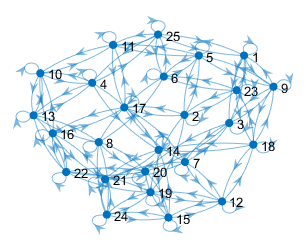
\includegraphics[scale=0.67]{img/Q4.png}}
    \subfigure[$Q_8$]
    {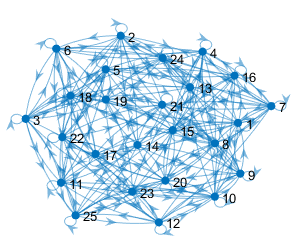
\includegraphics[scale=0.67]{img/Q8.png}}
    \subfigure[$Q_{12}$]
    {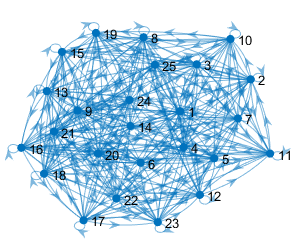
\includegraphics[scale=0.67]{img/Q12.png}}
    \subfigure[$Q_{18}$]
    {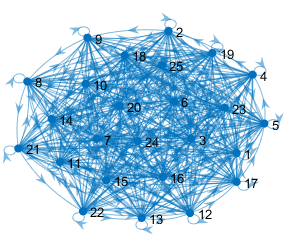
\includegraphics[scale=0.67]{img/Q18.png}}
    \caption{Topologies on which the analysis is conducted}
    \label{fig:Graphs}
\end{figure}
\begin{table}[h]\label{table:2}
    \centering
    \begin{tabular}{| p{3.5cm} | p{5.5cm} |p{2cm} |p{5cm} | }
        \hline
        \textbf{TOPOLOGY (Q)}&\textbf{EIGENVALUES $\vert \lambda_i \vert$}&\textbf{\texttt{esr}(Q)}&\textbf{CONVERGENCY TIME}\\
        \hline
        {\Large  $Q_4$}&{\small
            0.0450 ...
    0.7785
    \underline{1.0000}
        }&      {0.7785}&       { 10278}\\
        \hline
        {\Large  $Q_8$}&{\small
            0.0058 ...
    0.4964
    \underline{1.0000}
        }&    { 0.4964}&{ 10498}\\
        \hline
        {\Large $Q_{12}$}&{\small
            0.0053 ...
    0.3701
    \underline{1.0000}
        }&  { 0.3701}&{  10401}\\
        \hline
        {\Large  $Q_{18}$}&{\small
            0.0096 ...
        0.2196
        \underline{1.0000}}&   { 0.2196}&{10637}\\
        \hline
    \end{tabular}
    \caption{Main results for the analysis of the four topologies}
\end{table}

\noindent
The four matrices associated with the proposed topologies in Figure (2) have eigenvalues which satisfy the Perron-Frobenius Theorem since all are in magnitude less than $\lambda_{PF}=1$, then they reach consensus. Moreover, since the matrices are even \textbf{doubly stochastic} the system reaches the \textit{average consensus}.
About the \textbf{convergency} we can state that a smaller value for the essential spectral radius is associated with an higher number of needed iterations to converge. This information is summarized in the Table (2) 

\begin{wrapfigure}{r}{0.35\linewidth}
    \vspace{-0.3cm}
    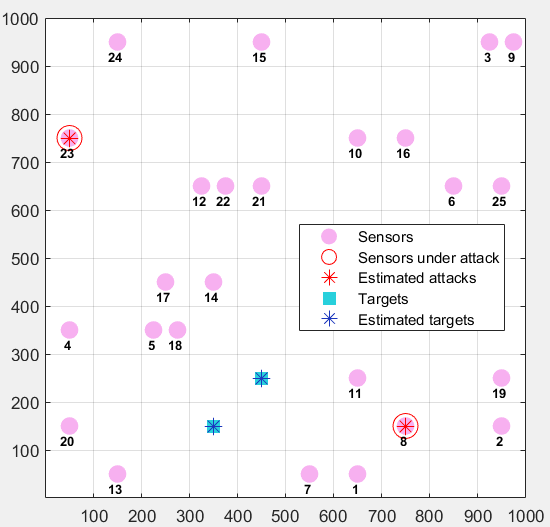
\includegraphics[width=0.9\linewidth]{img/Room.png} 
    \caption{Sensors, Target, estimates}
    \label{fig:Room}
\end{wrapfigure}
Furthermore, The algorithm has a \textbf{good accuracy} since the estimate for both the support for the target position (progressive number of the cells) and sensors under attack are correct, the Figure (\ref{fig:Room}) shows this result.
Another consideration can be done on the entries of the stochastic matrices. In particular, trying to change the magnitude of the entries $Q_{ij}$ there are not big differences on the convergency time. However in some situtions can be useful taking into account the weight of the edges. For example, let us suppose that on a link there is an attack in the sense that a certain sensor spread the measurement of the state corrupted by a quantity $a$, in that situation can be crucial - for the Secure State Estimation - the reduction of the quantity $Q_{ij}$ associated with the link under attack.

%----------------------------------------------       % Carlo Migliaccio    
\end{document}